
\chapter{Markov Decision Process}

% https://trunghng.github.io/artificial-intelligent/reinforcement-learning/2021/06/27/mdp-bellman-eqn.html

待重读的资源:
\begin{itemize}
%\setlength{\itemsep}{0pt}
%\setlength{\parsep}{0pt}
\setlength{\parskip}{0pt}
\item[-]
\url{http://www.cs.tulane.edu/~zzheng3/teaching/cmps6660/fall20/mdp.pdf}

\item[-]
\url{https://people.eecs.berkeley.edu/~pabbeel/cs287-fa12/slides/mdps-exact-methods.pdf}

\item[-]
\url{https://gibberblot.github.io/rl-notes/single-agent/MDPs.html}
\end{itemize}


%+++++++++++++++++++++++++++++++++++++++++++
\subsection{What is Reinforcement Learning?}

Say, there is an unknown environment that we're trying to put an agent on. By 
interacting with the agent through taking actions that gives rise to rewards 
continually, the agent learns a policy that maximize the cumulative rewards.

Reinforcement Learning (RL), roughly speaking, is an area of Machine Learning 
that describes methods aimed to learn a good strategy (called policy) for the 
agent from experimental trials and relative simple feedback received. With the 
optimal policy, the agent is capable to actively adapt to the environment to
maximize future rewards.

%+++++++++++++++++++++++++++++++++++++++++++
\subsection{Return}

The goal of agent is to maximize the cumulative reward in the long run. In 
general, we seek to maximize the expected return.

\begin{definition} {\rm\bf (Return)}
The return $G_t$ is the total discounted reward from $t$
\begin{equation}
G_t=R_{t+1}+\gamma R_{t+2}+\gamma^2 R_{t+3}+\dots=\sum_{k=0}^{\infty}\gamma^k R_{t+k+1},
\end{equation}
where $\gamma\in[0,1]$ is called discount rate (or discount factor).
\end{definition}

The discount rate $\gamma$ determines the present value of future rewards: a 
reward received $k$ time steps in the future is worth only $\gamma^{k-1}$ times 
what it would be worth if it were received immediately. And also, it provides 
mathematical convenience since as $k\rightarrow\infty$ then $\gamma^k\rightarrow 0$.


%+++++++++++++++++++++++++++++++++++++++++++
\subsection{Policy}

Policy, which is denoted as $\pi$, is the behaviour function of the agent. $\pi$ 
is a mapping from states to probabilities of selecting each possible action. In 
other words, it lets us know which action to take in the current state $s$ and can 
be either deterministic or stochastic.

\begin{itemize}
%\setlength{\itemsep}{0pt}
%\setlength{\parsep}{0pt}
\setlength{\parskip}{0pt}
\item[-]
Deterministic policy:
$\quad\pi(s)=a$

\item[-]
Stochastic policy: 
$\quad\pi(a|s)=P(A_t=a|S_t=s)$

\end{itemize}


%+++++++++++++++++++++++++++++++++++++++++++
\subsection{Value Function}

Value function measures how good a particular state is (or how good it is to 
perform a given action in a given state).

\begin{definition} {\rm\bf (state-value function)}
The state-value function of a state $s$ under a policy $\pi$, denoted as $v_\pi(s)$, 
is the expected return starting from state $s$ and following $\pi$ thereafter:
\begin{equation}
v_\pi(s)=\mathbb{E}_\pi[G_t|S_t=s]
\end{equation}
\end{definition}

状态值函数 $v_\pi(s)$ 可以评价当前状态的好坏,每个状态的值不仅由当前状态决定还要由后面的状态决定,
所以状态的累计奖励求期望就可得出当前$s$的状态值函数 $v_\pi(s)$。

\begin{definition} {\rm\bf (action-value function)}
Similarly, we define the value of taking action a in state $s$ under a policy $\pi$, 
denoted as $q_\pi(s,a)$, as the expected return starting from $s$, taking the 
action $a$, and thereafter following policy $\pi$:
\begin{equation}
q_\pi(s,a)=\mathbb{E}_\pi[G_t|S_t=s,A_t=a]
\end{equation}
Since we follow the policy $\pi$, we have that
\begin{equation}
v_\pi(s)=\sum_{a\in\mathcal{A}}q_\pi(s,a)\pi(a|s)
\end{equation}
\end{definition}



%+++++++++++++++++++++++++++++++++++++++++++
\section{Markov Decision Processes}
%-------------------------------------------

{\bf Markov decision processes (MDPs)} formally describe an environment for RL. 
And almost all RL problems can be formalised as MDPs.

\begin{definition} {\rm\bf (MDP)}
A Markov Decision Process is a tuple $<\mathcal{S}, \mathcal{A}, \mathcal{P}, 
\mathcal{R}, \gamma>$
\begin{itemize}
%\setlength{\itemsep}{0pt}
%\setlength{\parsep}{0pt}
\setlength{\parskip}{0pt}
\item[-]
$\mathcal{S}$ is a set of states called state space

\item[-]
$\mathcal{A}$ is a set of actions called action space

\item[-]
$\mathcal{P}$ is a state transition probability matrix \\
$\mathcal{P}^a_{ss'}=P(S_{t+1}=s'|S_t=s,A_t=a)$

\item[-]
$\mathcal{R}$ is a reward function \\
$ \mathcal{R}^a_s=\mathbb{E}\left[R_{t+1}|S_t=s,A_t=a\right]$

\item[-]
$\gamma\in[0, 1]$ is a discount factor for future reward

\end{itemize}
\end{definition}


\begin{definition}\label{def_FMDP} {\rm\bf (FMDP)}
A Finite Markov Decision Process is given a tuple $<\mathcal{S}, \mathcal{A}, \mathcal{T}, 
\rho, \mathcal{R}, H, \gamma>$
\begin{itemize}
%\setlength{\itemsep}{0pt}
%\setlength{\parsep}{0pt}
\setlength{\parskip}{0pt}
\item[-]
Set of states $\mathcal{S}$

\item[-]
Set of actions $\mathcal{A}$

\item[-]
$\mathcal{T}: \mathcal{S}\times\mathcal{A}\times\mathcal{S}\times\{0,1,\ldots,H\}
\rightarrow [0,1]$ \\
$\mathcal{T}_t(s,a,s')=P(s_{t+1}=s'|s_t=s,a_t=a)$ \\
$T(\cdot \vert s,a)$ is the transition kernel

\item[-]
$\rho$ the initial state distribution

\item[-]
$R$: \mathcal{S}\times\mathcal{A}\times\mathcal{S}\times\{0,1,\ldots,H\}
\rightarrow \mathcal{R} \\
$R_t(s,a,s')=\text{reward for} (s_{t+1}=s', s_t=s, a_t=a)$

\item[-]
$H$: horizon over which the agent will act

\item[-]
$\gamma\in[0, 1]$ is a discount factor for future reward

\end{itemize}
\end{definition}

Goal: Find $\pi: \mathcal{S}\times\{0,1,\ldots,H\}\rightarrow \mathcal{A}$ that 
maximizes expected sum of rewards, i.e., 
$$
\pi^*=\arg\max_\pi E\left[ \sum_{t=0}^H R_t(s_t, a_t, s_{t+1}) | \pi \right]
$$


%+++++++++++++++++++++++++++++++++++++++++++
\subsection{Optimal Policy and Optimal Value Function}

For finite MDPs (finite state and action space), we can precisely define an 
optimal policy. Value functions define a partial ordering over policies. A 
policy $\pi$ is defined to be better than or equal to a policy $\pi'$ if its 
expected return is greater than or equal to that of $\pi'$ for all states. In 
other words, 
\begin{equation} 
\pi\geq\pi'\iff v_\pi(s)\geq v_{\pi'} \forall s\in\mathcal{S} 
\end{equation}

\begin{theorem} {\rm\bf (Optimal policy)}
For any MDP, there exists an optimal policy $\pi_*$ that is better than or equal 
to all other policies, 
\begin{equation} 
\pi_*\geq\pi,\forall\pi 
\end{equation}
\end{theorem}

The proof of the above theorem is gonna be provided in another section since we 
need some additional tools to do that.

There may be more than one optimal policy, they share the same state-value function, 
called optimal state-value function though. 
\begin{equation} 
v_*(s)=\max_{\pi}v_\pi(s) 
\end{equation} 
Optimal policies also share the same action-value function, call optimal action-value 
function 
\begin{equation} 
q_*(s,a)=\max_{\pi}q_\pi(s,a) 
\end{equation}


%+++++++++++++++++++++++++++++++++++++++++++
\subsection{Bellman Equations}

A fundamental property of value functions used throughout RL is that they satisfy 
recursive relationships 
\begin{align*} 
v_\pi(s)&\doteq \mathbb{E}_\pi[G_t|S_t=s] \\
&=\mathbb{E}_\pi[R_t+\gamma G_{t+1}|S_t=s] \\
&=\sum_{s',r,g',a}p(s',r,g',a|s)(r+\gamma g') \\
&=\sum_{a}p(a|s)\sum_{s',r,g'}p(s',r,g'|a,s)(r+\gamma g') \\
&=\sum_{a}\pi(a|s)\sum_{s',r,g'}p(s',r|a,s)p(g'|s',r,a,s)(r+\gamma g') \\
&=\sum_{a}\pi(a|s)\sum_{s',r}p(s',r|a,s)\sum_{g'}p(g'|s')(r+\gamma g') \\
&=\sum_{a}\pi(a|s)\sum_{s',r}p(s',r|a,s)\left[r+\gamma\sum_{g'}p(g'|s')g'\right] \\
&=\sum_{a}\pi(a|s)\sum_{s',r}p(s',r|a,s)\left[r+\gamma v_\pi(s')\right], 
\end{align} 
where $p(s',r|s,a)=P(S_{t+1}=s',R_{t+1}=r|S_t=s,A_t=a)$, which defines the dynamics 
of the MDP. The last equation is called the Bellman equation for $v_\pi(s)$. It 
expresses a relationship between the value state $s$, $v_\pi(s)$ and the values of 
its successor states $s'$, $v_\pi(s')$.

Similarly, we define the Bellman equation for $q_\pi(s,a)$ 
\begin{align*} 
q_\pi(s,a)&\doteq\mathbb{E}_\pi[G_t|S_t=s,A_t=a] \\
&=\mathbb{E}_\pi[R_t+\gamma G_{t+1}|S_t=s,A_t=a] \\
&=\sum_{s',r}p(s',r|s,a)\left[r+\gamma\sum_{a'}\pi(a'|s')q_\pi(s',a')\right] 
\end{align}


%+++++++++++++++++++++++++++++++++++++++++++
\subsection{Bellman Backup Diagram}

Backup diagram of state-value function and action-value function respectively


\begin{tikzpicture}[->,>=stealth',level/.style={sibling distance = 5cm/#1,
  level distance = 1.5cm}] 
\node [arn_r] {}
    child{ node [arn_n] (test0) {}
        {
            child{ node [arn_r] {}
                {
                edge from parent node[above left] {$r$}
                edge from parent node[below left] (A) { \makebox[6em][l]{$v_\pi(s') \leftarrowtail s'$} }
                }
            }
            child{ node [arn_r] {} }
            edge from parent node[below left] (A) { \makebox[4em][l]{$a$} }
        }% edge from parent node[left] {$r$} %for a named pointer
    }
    child{ node [arn_n] (test1) {}
            child{ node [arn_r] {} }
            child{ node [arn_r] {} }
	}edge from parent node[left] (A) {\makebox[5em][l]{$v_\pi(s) \leftarrowtail s$}}
    
    ;

    %\filldraw[red] (A) circle[radius=1pt];
\end{tikzpicture}



\begin{tikzpicture}[->,>=stealth',level/.style={sibling distance = 5cm/#1,
  level distance = 1.5cm}] 
\node [arn_n] {}
    child{ node [arn_r] (test0) {}
        {
            child{ node [arn_n] {}
                {
                % edge from parent node[above left] {$r$}
                edge from parent node[below left] (A) { \makebox[8em][l]{$q_\pi(s',a') \leftarrowtail a'$} }
                }
            }
            child{ node [arn_n] {} }
            edge from parent node[below left] (A) { \makebox[4em][l]{$s'$} }
        } edge from parent node[left] {$r$} %for a named pointer
    }
    child{ node [arn_r] (test1) {}
            child{ node [arn_n] {} }
            child{ node [arn_n] {} }
	}edge from parent node[left] (A) {\makebox[7em][l]{$q_\pi(s,a) \leftarrowtail s, a$}}
    
    ;

    %\filldraw[red] (A) circle[radius=1pt];
\end{tikzpicture}


\subsection{Bellman Optimality Equations}

The optimal policy can be found once we have found the optimal state-value function 
$v_*$ and the optimal action-value function $q_*$.
Since $v_*$ is the value function for a policy, it must satisfy the Bellman equation 
for {\bf state-values}. Moreover, it is also the optimal value function, then we have 
\begin{align} 
v_*(s)&=\max_{a\in\mathcal{A}(s)}q_{\pi_*}(s,a)  \notag \\
&=\max_{a}\mathbb{E}_{\pi_*}[G_t|S_t=s,A_t=a]  \notag \\
&=\max_{a}\mathbb{E}_{\pi_*}[R_{t+1}+\gamma G_{t+1}|S_t=s,A_t=a]  \notag \\
&=\max_{a}\mathbb{E}[R_{t+1}+\gamma v_*(S_{t+1})|S_t=s,A_t=a]  \label{mdp_bellman_optimality_equation_1} \\
&=\max_{a}\sum_{s',r}p(s',r|s,a)[r+\gamma v_*(s')]  \label{mdp_bellman_optimality_equation_2}  
\end{align} 
The last two equations are two forms of the Bellman optimality equation for $v_*$. 
Similarly, we have the Bellman optimality equation for {\bf action-value} $q_*$ 
\begin{align} 
q_*(s,a)&=\mathbb{E}\left[R_{t+1}+\gamma\max_{a'}q_*(S_{t+1},a')|S_t=s,A_t=a\right] \\
&=\sum_{s',r}p(s',r|s,a)\left[r+\gamma\max_{a'}q_*(s',a')\right] 
\end{align}


\subsection{Bellman Optimality Equation vs Optimal Policy}
% https://yangyangfu.github.io/learning/reinforcement%20learning/2020/05/09/Bellman-Equation/

The ultimate goal of RL is to find the optimal policy. But how does the Bellman 
optimality equation relate to the optimal policy?

Once we find out the optimal state-value $v_*$, it is relatively easy to determine 
an optimal policy. For each state $s$, there will be one or more actions at which 
the maximum is obtained from the Bellman optimality equation. Any policy that assigns 
nonzero probability only to these actions is an optimal policy. You can think of this 
as a one-step search. If we have the optimal state-value function $v_*$, then the 
actions that appear best after a one-step search will be optimal actions.

Let's now retreat all these in another way: any policy that is greedy with respect to 
the optimal evaluation function $v_*$ is an optimal policy. The term greedy is used 
in computer science to describe any search or decision procedure that selects 
alternatives based only on local or immediate considerations, without considering the 
possibility that such a selection may prevent future access to even better alternatives. 
Consequently, it describes policies that select actions based only on their short-term 
consequences. The beauty of $v_*$ is that if one uses it to evaluate the short-term 
consequences of actions—specifically, the one-step consequences—then a greedy policy is 
actually optimal in the long-term sense in which we are interested because $v_*$ already 
takes into consideration the reward consequences of all possible future behavior. By 
means of $v_*$, the optimal expected long-term return is turned into a quantity that is 
locally and immediately available for each state. Hence, a one-step-ahead search yields 
the long-term optimal actions.

Having $q_*$ makes choosing optimal actions even easier. With $q_*$, the agent does not 
even have to do a one-step-ahead search: for any state $s$, it can simply find any 
action that maximizes $q_*(s, a)$. The action-value function actively caches the results 
of all one-step-ahead searches. It provides the optimal expected long-term return as a 
value that is locally and immediately available for each state–action pair. Hence at the 
cost of representing a function of state–action pairs, instead of just of states, the 
optimal actionvalue function allows optimal actions to be selected without having to 
know anything about possible successor states and their values, that is, without having 
to know anything about the environment's dynamics.



\subsection{Backup diagram for $v_*$ and $q_*$}


\begin{figure}[H]
\centering
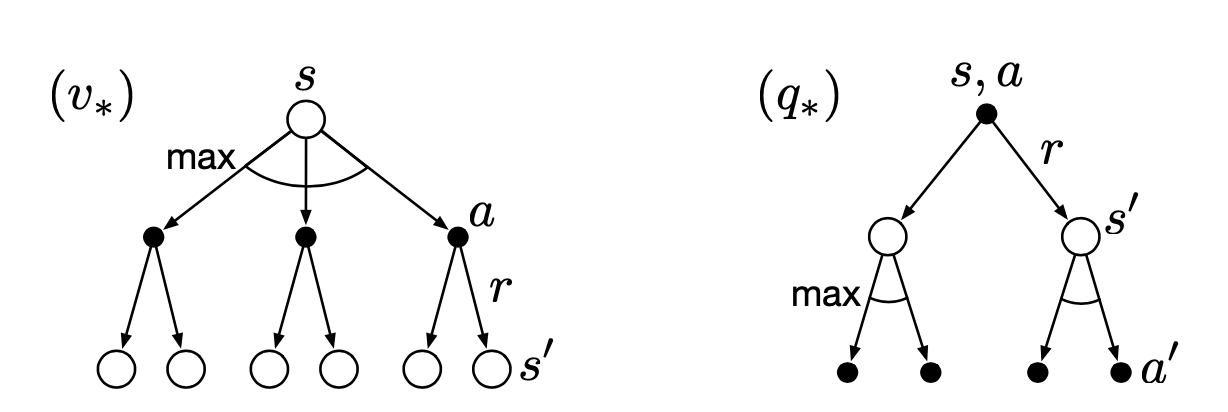
\includegraphics[scale=0.618]{pix/opt.png}
\caption{backup diagram for $v_*$ and $q_*$}
%\label{fig:label}
\end{figure}


\subsection{References}

\cite{silver2015}

% https://lilianweng.github.io/lil-log/2018/02/19/a-long-peek-into-reinforcement-learning.html

% https://deepmind.com/research/case-studies/alphago-the-story-so-far


\section{Canonical Example: Grid World}

\begin{itemize}
%\setlength{\itemsep}{0pt}
%\setlength{\parsep}{0pt}
\setlength{\parskip}{0pt}
\item
The agent lives in a grid, figure \ref{fig:mdp_Grid_world}

\item
Walls block the agent's path

\item
The agent's actions do not always go as planned:
    \begin{itemize}
    \item
    $80\%$ of the time, the action North takes the agent North(if there is no wall there)

    \item
    $10\%$ of the time, North takes the agent West; $10\%$ East

    \item
    If there is a wall in the direction the agent would have been taken, the agent stays put

    \end{itemize}

\item
Big rewards come at the end

\end{itemize}

\begin{figure}[H]
\centering
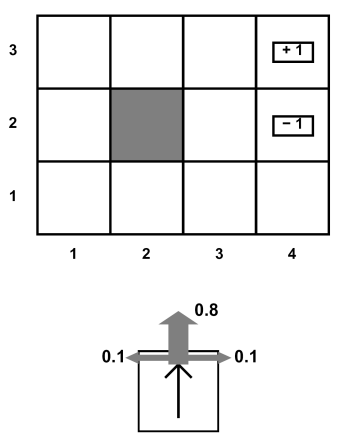
\includegraphics[scale=0.618]{pix/mdp/Grid_world.png}
\caption{Canonical Example: Grid world}
\label{fig:mdp_Grid_world}
\end{figure}

{\bf Solving MDPs}

\begin{itemize}
\item
In an MDP, we want an optimal \textcolor{red}{policy $\pi^*: S\times 0: H\rightarrow A$}

    \begin{itemize}
    \item
    A policy $\pi$ gives an action for each state for each time, figure \ref{fig:action_for_each_state}

    \begin{figure}[H]
    \centering
    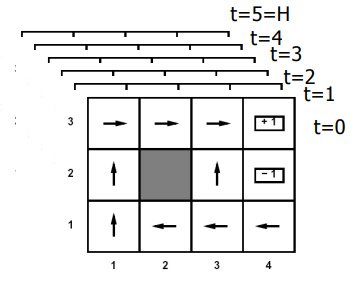
\includegraphics[scale=0.618]{pix/mdp/action_for_each_state.png}
    \caption{Canonical Example: action for each state}
    \label{fig:action_for_each_state}
    \end{figure}

    \item
    An optimal policy maximizes expected sum of rewards

    \end{itemize}

\item
Contrast: In deterministic, want an optimal \textcolor{magenta}{plan}, or sequence 
of actions, from start to a goal
\end{itemize}

Optimal Control

$=$

given an MDP $(\mathcal{S}, \mathcal{A}, \mathcal{T}, \mathcal{R}, \gamma, H)$

find the optimal policy $\pi^*$

Exact Methods:
\begin{itemize}
\item
Value Iteration

\item
Policy Iteration

\item
Linear Programming
\end{itemize}


\subsection{Value iteration}

Algorithm:
\begin{itemize}
\item
Start with $V_0^*(s)=0$ for all $s$.

\item
For $i=1,\ldots, H$ \\
Given $V_i^*$, calculate for all states $s\in\mathcal{S}$: \\
\textcolor{magenta}{
$$
V_{i+1}^*(s) \leftarrow \max_a\sum_{s'}T(s,a,s')\left[
R(s,a,s') + V_i^*(s') \right]
$$
}

\item
This is called a \textcolor{magenta}{value update} or \textcolor{magenta}{
Bellman update/back-up}
\end{itemize}

\noindent where $V_i^*(s)$ is the expected sum of rewards accumulated when 
starting from state $s$ and acting optimally for 
\textcolor{red}{\bf a horizon of $i$ steps}


\subsection{Value iteration in Gridworld}

$\text{noise} = 0.2$, $\gamma=0.9$, two terminal states with $R=+1$ and $-1$. 

\begin{figure}[hp]
\centering
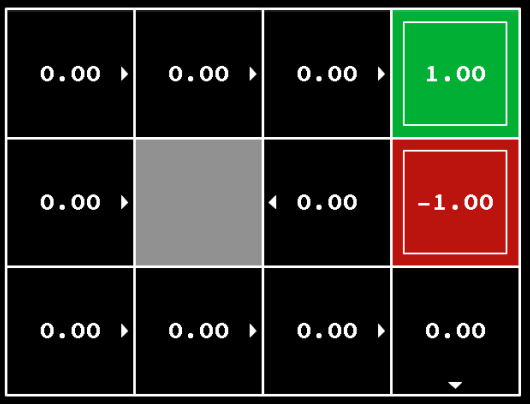
\includegraphics[scale=0.618]{pix/mdp/grid_world_value_iteration_1.png}
\caption{Grid World: Values after 1 iteration}
%\label{fig:action_for_each_state}
\end{figure}

\begin{figure}[hp]
\centering
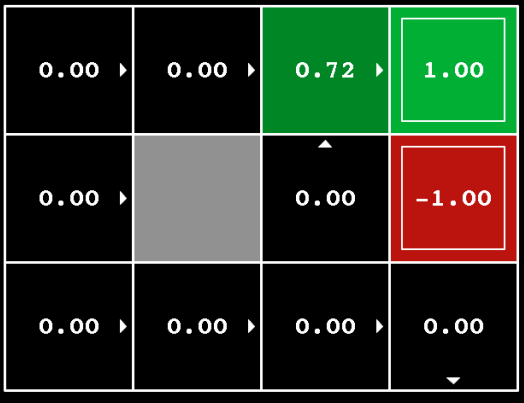
\includegraphics[scale=0.618]{pix/mdp/grid_world_value_iteration_2.png}
\caption{Grid World: Values after 2 iterations}
%\label{fig:action_for_each_state}
\end{figure}

\begin{figure}[hp]
\centering
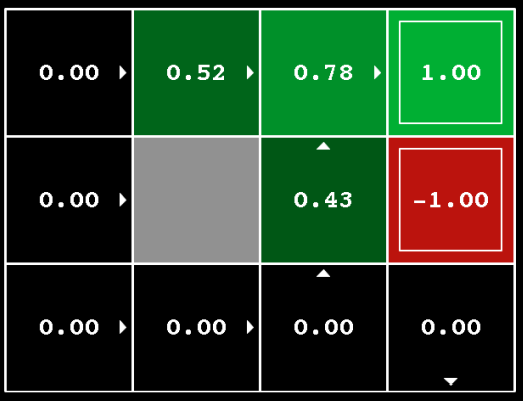
\includegraphics[scale=0.618]{pix/mdp/grid_world_value_iteration_3.png}
\caption{Grid World: Values after 3 iterations}
%\label{fig:action_for_each_state}
\end{figure}

\begin{figure}[hp]
\centering
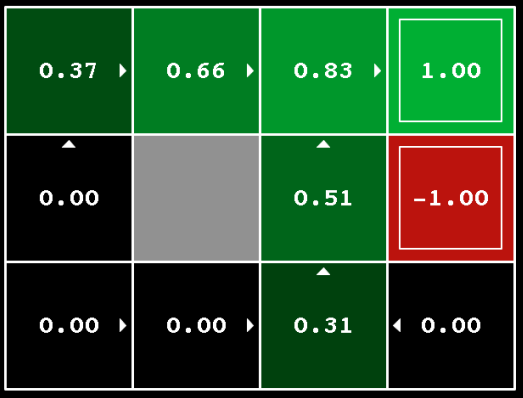
\includegraphics[scale=0.618]{pix/mdp/grid_world_value_iteration_4.png}
\caption{Grid World: Values after 4 iterations}
%\label{fig:action_for_each_state}
\end{figure}

\begin{figure}[hp]
\centering
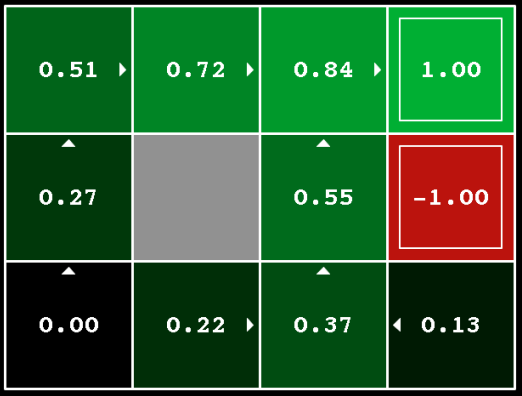
\includegraphics[scale=0.618]{pix/mdp/grid_world_value_iteration_5.png}
\caption{Grid World: Values after 5 iterations}
%\label{fig:action_for_each_state}
\end{figure}

\begin{figure}[hp]
\centering
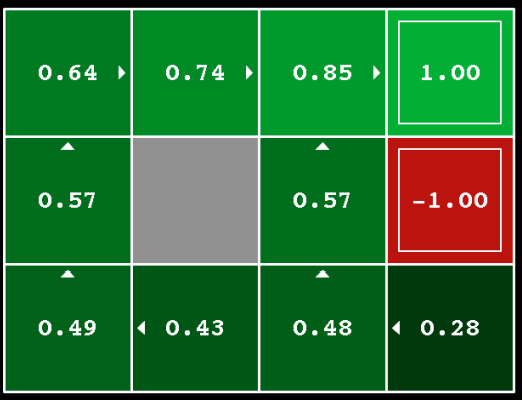
\includegraphics[scale=0.618]{pix/mdp/grid_world_value_iteration_100.png}
\caption{Grid World: Values after 100 iterations}
%\label{fig:action_for_each_state}
\end{figure}

\begin{figure}[hp]
\centering
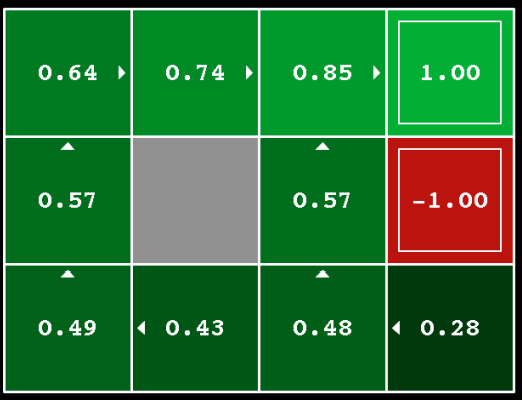
\includegraphics[scale=0.618]{pix/mdp/grid_world_value_iteration_100.png}
\caption{Grid World: Values after 1000 iterations}
%\label{fig:action_for_each_state}
\end{figure}

{\bf \textcolor{magenta}{当前进展总结:}}
\begin{itemize}
%\setlength{\itemsep}{0pt}
%\setlength{\parsep}{0pt}
\setlength{\parskip}{0pt}
\item[-]
当前能正确运行的代码的位置 $D:/mygit/reinforcement\_mdp/gridworld.py$

\item[-]
参数的设置位于 gridworld.py 的 ln494 及之后的一段

\item[-]
代码的来源及说明参见(修改后的代码运行结果经过检测满足Question 1的要求) \\
\url{https://courses.cs.washington.edu/courses/csep573/19wi/assignments/reinforcement_mdp.html}
\\
网页被另存于本地位置 \\
\url{file:///D:/webPages/mdp/Assignment%203_%20Markov%20Decision%20Processes%20-%20CSE%20P%20573.html}

\item[-]
代码修改的依据参见 \\
\url{https://gitee.com/industry-ai/mdp}

\end{itemize}


\subsection{Example Analysis}

% https://hub.packtpub.com/reinforcement-learning-mdp-markov-decision-process-tutorial/

The Markov decision process, better known as MDP, is an approach in reinforcement 
learning to take decisions in a gridworld environment. A gridworld environment 
consists of states in the form of grids.

The MDP tries to capture a world in the form of a grid by dividing it into states, 
actions, models/transition models, and rewards. The solution to an MDP is called 
a policy and the objective is to find the optimal policy for that MDP task.

Thus, any reinforcement learning task composed of a set of states, actions, and 
rewards that follows the Markov property would be considered an MDP.

In this subsection, we will dig deep into MDPs, states, actions, rewards, policies, 
and how to solve them using Bellman equations through the above gridworld example.

\subsubsection{Markov decision processes}

这里复习一下MDP的定义 \ref{def_FMDP}

MDP is defined as the collection of the following:
\begin{itemize}
%\setlength{\itemsep}{0pt}
%\setlength{\parsep}{0pt}
\setlength{\parskip}{0pt}
\item[-]
{\bf States:} $\mathcal{S}$

\item[-]
{\bf Actions:} $\mathcal{A}$

\item[-]
{\bf Transition model:} $\mathcal{T}: \mathcal{S}\times\mathcal{A}\times\mathcal{S}\times\{0,1,\ldots,H\}
\rightarrow [0,1]$ \\
$\mathcal{T}_t(s,a,s')=P(s_{t+1}=s'|s_t=s,a_t=a)$ \\
$T(s,a,s')\sim P(s'|s,a)$ 

\item[-]
{\bf Rewards:} $R$: \mathcal{S}\times\mathcal{A}\times\mathcal{S}\times\{0,1,\ldots,H\}
\rightarrow \mathcal{R} \\
$R_t(s,a,s')=\text{reward for} (s_{t+1}=s', s_t=s, a_t=a)$ \\
$R(s), R(s,a), R(s,a,s')$

\item[-]
{\bf Policy:} 
$\pi: \mathcal{S}\times\{0,1,\ldots,H\}\rightarrow \mathcal{A}$ \\
$\pi(s) \rightarrow a$ \\
$\pi^*$ is the optimal policy

\end{itemize}

In the case of an MDP, the environment is fully observable, that is, whatever 
observation the agent makes at any point in time is enough to make an optimal 
decision. In case of a partially observable environment, the agent needs a 
memory to store the past observations to make the best possible decisions.

Let's try to break this into different lego blocks to understand what this 
overall process means.

\subsubsection{The Markov property}

In short, as per the {\bf Markov property}, in order to know the information 
of near future (say, at time $t+1$) the present information at time $t$ matters.

Given a sequence, $[x_1, x_2, \ldots, x_t]$, the first order of Markov says,
$P(x_t | x_{t-1}, x_{t-2}, \ldots, x_1) = P(x_t | x_{t-1})$, that is,
$x_t$ depends only on $x_{t-1}$. Therefore, $x_{t+1}$ will depend only on $x_t$. 
The second order of Markov says, $P(x_t | x_{t-1}, x_{t-2}, \ldots, x_1) = 
P(x_t | x_{t-1}, x_{t-2})$, that is, $x_t$ depends only on $x_{t-1}$ and 
$x_{t-2}$.

In our context, we will follow the first order of the Markov property from now 
on. Therefore, we can convert any process to a Markov property if the probability 
of the new state, say $x_{t+1}$, depends only on the current state, $x_t$, such 
that the current state captures and remembers the property and knowledge from the 
past. Thus, as per the Markov property, the world (that is, the environment) is 
considered to be stationary, that is, the rules in the world are fixed.

\subsubsection{The state set}

The state set $\mathcal{S}$ is a set of different states, which constitute the 
environment. States are the feature representation of the data obtained from the 
environment. Thus, any input from the agent's sensors can play an important role 
in state formation. State spaces can be either discrete or continuous. The starts 
from start state and has to reach the goal state in the most optimized path without 
ending up in bad states (like the red colored state shown in the diagram below).

Consider the following gridworld as having 12 discrete states, where the 
green-colored grid is the goal state, red is the state to avoid, and black is a 
wall that you'll bounce back from if you hit it head on:

\begin{figure}[H]
\centering
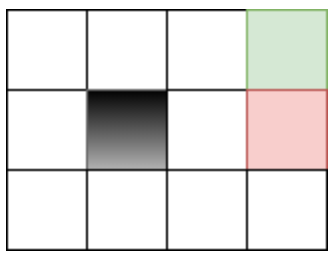
\includegraphics[scale=0.618]{pix/mdp/grid_world_states.png}
\caption{Grid World: states}
%\label{fig:action_for_each_state}
\end{figure}

The states can be represented as $1, 2, \ldots, 12$ or by coordinates, $(1,1),(1,2),
\ldots, (3,4)$.

\subsubsection{Actions}

The {\bf actions} are the things an agent can perform or execute in a particular 
state. In other words, actions are sets of things an agent is allowed to do in 
the given environment. Like states, actions can also be either discrete or continuous.

Consider the above gridworld example having 12 discrete states and 4 discrete 
actions ({\bf UP}, {\bf DOWN}, {\bf RIGHT}, and {\bf LEFT}).
The preceding example shows the action space to be a discrete set space, that is, 
$a\in \mathcal{A}$ where, $\mathcal{A} = \{\text{UP}, \text{DOWN}, \text{RIGHT},
\text{LEFT} \}$. It can also be treated as a function of state, that is, $a = A(s)$, 
where depending on the state function, it decides which action is possible.

\subsubsection{Transition model}

The transition model $T(s, a, s')$ is a function of three variables, which are the 
current state $s$, action $a$, and the new state $s'$, and defines the rules to 
play the game in the environment. It gives probability $P(s'|s, a)$, that is, the 
probability of landing up in the new $s'$ state given that the agent takes an action, 
$a$, in given state, $s$.

{\bf The transition model plays the crucial role in a stochastic world, unlike the case 
of a deterministic world where the probability for any landing state other than the 
determined one will have zero probability.}

Let's consider the above environment (world) and consider different cases, 
determined and stochastic:

Since the actions $a\in \mathcal{A}$ where, $\mathcal{A} = \{\text{UP}, \text{DOWN}, 
\text{RIGHT}, \text{LEFT} \}$.
The behavior of these two cases depends on certain factors:
\begin{itemize}
%\setlength{\itemsep}{0pt}
%\setlength{\parsep}{0pt}
\setlength{\parskip}{0pt}
\item[-]
{\bf Determined environment}: In a determined environment, if you take a certain 
action, say {\bf UP}, you will certainly perform that action with probability $1$.

\item[-]
{\bf Stochastic environment}: In a stochastic environment, if you take the same 
action, say {\bf UP}, there will certain probability say $0.8$ to actually perform 
the given action and there is $0.1$ probability it can perform an action (either 
{\bf LEFT} or {\bf RIGHT}) perpendicular to the given action, {\bf UP}. Here, for 
the $s$ state and the {\bf UP} action transition model, 
$T(s',\text{UP}, s) = P(s'| s,\text{UP}) = 0.8$.
\end{itemize}

Since $T(s,a,s') \sim P(s'|s,a)$, where the probability of new state depends on 
the current state and action only, and none of the past states. Thus, the 
transition model follows the first order Markov property.

We can also say that our universe is also a stochastic environment, since the 
universe is composed of atoms that are in different states defined by position 
and velocity. Actions performed by each atom change their states and cause 
changes in the universe.

\subsubsection{Rewards}

The {\bf reward} of the state quantifies the usefulness of entering into a state. 
There are three different forms to represent the reward namely, $R(s)$, $R(s, a)$ 
and $R(s, a, s')$, but they are all equivalent.

For a particular environment, the domain knowledge plays an important role in the 
assignment of rewards for different states as minor changes in the reward do 
matter for finding the optimal solution to an MDP problem.

There are two approaches we reward our agent for when taking a certain action. 
They are:
\begin{itemize}
%\setlength{\itemsep}{0pt}
%\setlength{\parsep}{0pt}
\setlength{\parskip}{0pt}
\item[-]
{\bf Credit assignment problem}: We look at the past and check which actions led 
to the present reward, that is, which action gets the credit

\item[-]
{\bf Delayed rewards}: In contrast, in the present state, we check which action 
to take that will lead us to potential rewards
\end{itemize}

Delayed rewards form the idea of foresight planning. Therefore, this concept is 
being used to calculate the expected reward for different states. We will discuss 
this in the later subsections.

\subsubsection{Policy}

Until now, we have covered the blocks that create an MDP problem, that is, states, 
actions, transition models, and rewards, now comes the solution. The policy is 
the solution to an MDP problem.

\noindent{Policy:} $\pi(s) \rightarrow a$

The policy is a function that takes the state as an input and outputs the action 
to be taken. Therefore, the policy is a command that the agent has to obey.

$\pi^*$ is called the optimal policy, which maximizes the expected reward. Among 
all the policies taken, the optimal policy is the one that optimizes to maximize 
the amount of reward received or expected to receive over a lifetime. For an MDP, 
there's no end of the lifetime and you have to decide the end time.

Thus, the policy is nothing but a guide telling which action to take for a given 
state. It is not a plan but uncovers the underlying plan of the environment by 
returning the actions to take for each state.

\subsubsection{The Bellman equations}

Since the optimal $\pi^*$ policy is the policy that maximizes the expected rewards, 
therefore, 
$$
\pi^*=\arg\max_\pi E\left[ \sum_{t=0}^\infty \gamma^tR(s_t) | \pi \right],
$$
\noindent{where} $E\left[ \sum_{t=0}^\infty \gamma^tR(s_t) | \pi \right]$ means the 
expected value of the rewards obtained from the sequence of states agent observes 
if it follows the $\pi$ policy. Thus, $\arg\max_\pi$ outputs the $\pi$ policy that 
has the highest expected reward.

Similarly, we can also calculate the {\bf utility of the policy of a state}, that 
is, if we are at the state $s$, given a policy $\pi$, then, the utility of the 
policy $pi$ for the state $s$, that is, $U^\pi(s)$ would be the expected rewards 
from that state onward:
$$
U^\pi(s) = E\left[ \sum_{t=0}^\infty \gamma^tR(s_t) | \pi, s_0 = s \right],
$$
\noindent{The} immediate reward of the state, that is, $R(s)$ is different than the 
utility of the $U(s)$ state (that is, the utility of the optimal policy of the 
$U^{\pi^*}(s)$ state) because of the concept of delayed rewards. From now on, the 
utility of the $U(s)$ state will refer to the utility of the optimal policy of the 
state, that is, the U^{\pi^*}(s)$ state.

Moreover, the optimal policy can also be regarded as the policy that maximizes the 
expected utility. Therefore,
$$
\pi^*=\arg\max_a \sum_{s'} T(s,a,s')U(s')
$$
\noindent{where}, $T(s,a,s')$ is the transition probability, that is, $P(s'|s,a)$ 
and $U(s')$ is the utility of the new landing state after the action $a$ is taken on 
the state $s$. $\sum_{s'} T(s,a,s')U(s')$ refers to the summation of all possible 
new state outcomes for a particular action taken, then whichever action gives the 
maximum value of $\pi^*=\arg\max_a \sum_{s'} T(s,a,s')U(s')$ that is considered to 
be the part of the optimal policy and thereby, the utility of the state $s'$ is 
given by the following Bellman equation,

\begin{equation}\label{mdp_bellman_equation}
U(s) = R(s) + \gamma\max_a \sum_{s'} T(s,a,s')U(s')
\end{equation}

\noindent{where}, $R(s)$ is the immediate reward and $\max_a \sum_{s'} T(s,a,s')U(s')$ 
is the reward from future, that is, the discounted utilities of the state $s'$ where 
the agent can reach from the given $s$ state if the action, $a$, is taken.


\subsubsection{Solving the Bellman equation to find policies}

Say we have some $n$ states in the given environment and if we see the Bellman 
equation \ref{mdp_bellman_equation} we find out that $n$ states are given; therefore, 
we will have $n$ equations and $n$ unknown but the $\max_a$ function makes it 
non-linear. Thus, we cannot solve them as linear equations.

Therefore, in order to solve:

\begin{itemize}
%\setlength{\itemsep}{0pt}
%\setlength{\parsep}{0pt}
\setlength{\parskip}{0pt}
\item[-]
Start with an arbitrary utility

\item[-]
Update the utilities based on the neighborhood until convergence, that is, update 
the utility of the state using the Bellman equation based on the utilities of the 
landing states from the given state
\end{itemize}

Iterate this multiple times to lead to the true value of the states. This process 
of iterating to convergence towards the true value of the state is called value 
iteration.

For the terminal states where the game ends, the utility of those terminal state 
equals the immediate reward the agent receives while entering the terminal state.

Let's try to understand this by implementing an example.


%+++++++++++++++++++++++++++++++++++++++++++
\subsection{An example of value iteration using the Bellman equation}

Consider the following environment and the given information:

\begin{figure}[H]
\centering
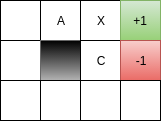
\includegraphics[scale=0.618]{pix/mdp/grid_world_acx.png}
\caption{Grid World: ACX}
%\label{fig:action_for_each_state}
\end{figure}

Given information:
\begin{itemize}
%\setlength{\itemsep}{0pt}
%\setlength{\parsep}{0pt}
\setlength{\parskip}{0pt}
\item[-]
$A$, $C$, and $X$ are the names of some states.

\item[-]
The green-colored state is the goal state, $G$, with a reward of $+1$.

\item[-]
The red-colored state is the bad state, $B$, with a reward of $-1$, try to 
prevent your agent from entering this state

\item[-]
Thus, the green and red states are the terminal states, enter either and the 
game is over. If the agent encounters the green state, that is, the goal state, 
the agent wins, while if they enter the red state, then the agent loses the game.

\item[-]
$\gamma=1/2$, $R(s)=-0.04$ (that is, reward for all states except the $G$ and $B$ 
states is $-0.04$),  (that is, the utility at the first time step is $0$, except 
the $G$ and $B$ states).

\item[-]
Transition probability $T(s,a,s')$ equals $0.8$ if going in the desired direction; 
otherwise, $0.1$ each if going perpendicular to the desired direction. For example, 
if the action is UP then with $0.8$ probability, the agent goes UP but with $0.1$ 
probability it goes RIGHT and $0.1$ to the LEFT.
\end{itemize}

Questions:

\begin{itemize}
%\setlength{\itemsep}{0pt}
%\setlength{\parsep}{0pt}
\setlength{\parskip}{0pt}
\item[1.]
Find $U_1(X)$, the utility of the $X$ state at time step $1$, that is, the agent 
will go through one iteration

\item[2.]
Similarly, find $U_2(X)$.
\end{itemize}

Solution:

\begin{align*}
U_0(X) &= 0 \\
U_1(X) &= R(X) + \gamma\max_a\sum_{s'} T(s,a,s') U_0(s') \\
R(X) &= -0.04
\end{align}

\begin{table}[H]   
\begin{center}   
%\caption{title}  
%\label{table:1} 
\begin{tabular}{|c|c|c|c|c|}   
\hline   Action $a$ & $s'$ & $T(s,a,s')$ & $U_0(s')$ & $T(s,a,s')U_0(s')$ \\   
\hline   RIGHT & G & $0.8$ & $+1$ & $0.8\times 1=0.8$ \\ 
\hline   RIGHT & C & $0.1$ & $0$ & $0.1\times 0=0$ \\  
\hline   RIGHT & X & $0.1$ & $0$ & $0.1\times 0=0$ \\
\hline
\end{tabular}   
\end{center}   
\end{table}

Thus, for action $a = \text{RIGHT}$,
$$
\left[\sum_{s'} T(s,a,s') U_0(s') = 0.8 + 0 + 0 = 0.8\right]_{\text{right}}
$$


\begin{table}[H]   
\begin{center}   
%\caption{title}  
%\label{table:1} 
\begin{tabular}{|c|c|c|c|c|}   
\hline   Action $a$ & $s'$ & $T(s,a,s')$ & $U_0(s')$ & $T(s,a,s')U_0(s')$ \\   
\hline   DOWN & C & $0.8$ & $0$ & $0.8\times 0=0$ \\ 
\hline   DOWN & G & $0.1$ & $+1$ & $0.1\times 1=0.1$ \\  
\hline   DOWN & A & $0.1$ & $0$ & $0.1\times 0=0$ \\
\hline
\end{tabular}   
\end{center}   
\end{table}

Thus, for action $a = \text{DOWN}$,
$$
\left[\sum_{s'} T(s,a,s') U_0(s') = 0 + 0.1 + 0 = 0.1\right]_{\text{down}}
$$


\begin{table}[H]   
\begin{center}   
%\caption{title}  
%\label{table:1} 
\begin{tabular}{|c|c|c|c|c|}   
\hline   Action $a$ & $s'$ & $T(s,a,s')$ & $U_0(s')$ & $T(s,a,s')U_0(s')$ \\   
\hline   UP & X & $0.8$ & $0$ & $0.8\times 0=0$ \\ 
\hline   UP & G & $0.1$ & $+1$ & $0.1\times 1=0.1$ \\  
\hline   UP & A & $0.1$ & $0$ & $0.1\times 0=0$ \\
\hline
\end{tabular}   
\end{center}   
\end{table}

Thus, for action $a = \text{UP}$,
$$
\left[\sum_{s'} T(s,a,s') U_0(s') = 0 + 0.1 + 0 = 0.1\right]_{\text{up}}
$$


\begin{table}[H]   
\begin{center}   
%\caption{title}  
%\label{table:1} 
\begin{tabular}{|c|c|c|c|c|}   
\hline   Action $a$ & $s'$ & $T(s,a,s')$ & $U_0(s')$ & $T(s,a,s')U_0(s')$ \\   
\hline   LEFT & A & $0.8$ & $0$ & $0.8\times 0=0$ \\ 
\hline   LEFT & X & $0.1$ & $0$ & $0.1\times 0=0$ \\  
\hline   LEFT & C & $0.1$ & $0$ & $0.1\times 0=0$ \\
\hline
\end{tabular}   
\end{center}   
\end{table}

Thus, for action $a = \text{LEFT}$,
$$
\left[\sum_{s'} T(s,a,s') U_0(s') = 0 + 0 + 0 = 0\right]_{\text{left}}
$$

Therefore, among all actions,
$$
\max_a \sum_{s'} T(s,a,s') U_0(s') = 
\left[\sum_{s'} T(s,a,s') U_0(s') = 0.8 + 0 + 0 = 0.8\right]_{\text{right}}
= 0.8
$$

Therefore,
$$
U_1(X) = -0.04 + 0.5 \times 0.8 = 0.36,
$$
\noindent{where} $R(X) = -0.04$ and $\gamma=1/2=0.5$.

Similarly, we calculate to get
$U_1(A) = -0.04$ and $U_1(C) = -0.04$.

Since,
$U_1(X) = 0.36$, $U_1(A) = -0.04$, $U_1(C) = -0.04$, $U_1(G)=1$, $U_1(B)=-1$,
and, $U_2(X) = R(X) + \gamma\max_a \sum_{s'} T(s,a,s')U_1(s')$, $R(X)=-0.04$

\begin{table}[H]   
\begin{center}   
%\caption{title}  
%\label{table:1} 
\begin{tabular}{|c|c|c|c|c|}   
\hline   Action $a$ & $s'$ & $T(s,a,s')$ & $U_1(s')$ & $T(s,a,s')U_1(s')$ \\   
\hline   RIGHT & G & $0.8$ & $+1$ & $0.8\times 1=0.8$ \\ 
\hline   RIGHT & C & $0.1$ & $-0.04$ & $0.1\times -0.04=-0.004$ \\  
\hline   RIGHT & X & $0.1$ & $0.36$ & $0.1\times 0.36=0.036$ \\
\hline
\end{tabular}   
\end{center}   
\end{table}

Thus, for action $a = \text{RIGHT}$,
$$
\left[\sum_{s'} T(s,a,s') U_1(s') = 0.8 - 0.004 + 0.036 = 0.832\right]_{\text{right}}
$$

\begin{table}[H]   
\begin{center}   
%\caption{title}  
%\label{table:1} 
\begin{tabular}{|c|c|c|c|c|}   
\hline   Action $a$ & $s'$ & $T(s,a,s')$ & $U_1(s')$ & $T(s,a,s')U_1(s')$ \\   
\hline   DOWN & C & $0.8$ & $-0.04$ & $0.8\times -0.04=-0.032$ \\ 
\hline   DOWN & G & $0.1$ & $+1$ & $0.1\times 1=0.1$ \\  
\hline   DOWN & A & $0.1$ & $-0.04$ & $0.1\times -0.04=-0.004$ \\
\hline
\end{tabular}   
\end{center}   
\end{table}

Thus, for action $a = \text{DOWN}$,
$$
\left[\sum_{s'} T(s,a,s') U_1(s') = -0.032 + 0.1 - 0.004 = 0.064\right]_{\text{down}}
$$

\begin{table}[H]   
\begin{center}   
%\caption{title}  
%\label{table:1} 
\begin{tabular}{|c|c|c|c|c|}   
\hline   Action $a$ & $s'$ & $T(s,a,s')$ & $U_1(s')$ & $T(s,a,s')U_1(s')$ \\   
\hline   UP & X & $0.8$ & $0.36$ & $0.8\times 0.36=0.288$ \\ 
\hline   UP & G & $0.1$ & $+1$ & $0.1\times 1=0.1$ \\  
\hline   UP & A & $0.1$ & $-0.04$ & $0.1\times -0.04=-0.004$ \\
\hline
\end{tabular}   
\end{center}   
\end{table}

Thus, for action $a = \text{UP}$,
$$
\left[\sum_{s'} T(s,a,s') U_1(s') = 0.288 + 0.1 - 0.004 = 0.384\right]_{\text{up}}
$$

\begin{table}[H]   
\begin{center}   
%\caption{title}  
%\label{table:1} 
\begin{tabular}{|c|c|c|c|c|}   
\hline   Action $a$ & $s'$ & $T(s,a,s')$ & $U_1(s')$ & $T(s,a,s')U_1(s')$ \\   
\hline   LEFT & A & $0.8$ & $-0.04$ & $0.8\times -0.04=-0.032$ \\ 
\hline   LEFT & X & $0.1$ & $0.36$ & $0.1\times 0.36=0.036$ \\  
\hline   LEFT & C & $0.1$ & $-0.04$ & $0.1\times -0.04=-0.004$ \\
\hline
\end{tabular}   
\end{center}   
\end{table}

Thus, for action $a = \text{LEFT}$,
$$
\left[\sum_{s'} T(s,a,s') U_1(s') = -0.032 + 0.036 - 0.004 = 0\right]_{\text{left}}
$$

Therefore, among all actions,
$$
\max_a \sum_{s'} T(s,a,s') U_1(s') = 
\left[\sum_{s'} T(s,a,s') U_1(s') = 0.8 - 0.004 + 0.036 = 0.832\right]_{\text{right}}
= 0.832
$$

Therefore,
$$
U_2(X) = -0.04 + 0.5 \times 0.832 = 0.376,
$$
\noindent{where} $R(X) = -0.04$ and $\gamma=1/2=0.5$.

Therefore, the answers to the preceding questions are:
\begin{itemize}
%\setlength{\itemsep}{0pt}
%\setlength{\parsep}{0pt}
\setlength{\parskip}{0pt}
\item[1.]
$U_1(X) = 0.36$

\item[2.]
$U_2(X) = 0.376$
\end{itemize}


\subsubsection{Policy iteration}

The process of obtaining optimal utility by iterating over the policy and updating 
the policy itself instead of value until the policy converges to the optimum is 
called policy iteration. The process of policy iteration is as follows:
\begin{itemize}
%\setlength{\itemsep}{0pt}
%\setlength{\parsep}{0pt}
\setlength{\parskip}{0pt}
\item[-]
Start with a random policy, $\pi_0$

\item[-]
For the given $\pi_t$ policy at iteration step $t$, calculate $U_t=U_t^\pi$ by 
using the following formula: \\
$U_t(s) &= R(s) + \gamma\max_a\sum_{s'} T(s,\pi_t(s),s') U_{t-1}(s')$

\item[-]
Improve the $\pi_{t+1}$ policy by \\
$\pi_{t+1} = \arg\max_a\sum_{s'} T(s,a,s')U_t(s')$
\end{itemize}

Here ends an interesting MDP example calculation.


%+++++++++++++++++++++++++++++++++++++++++++
\section{Control as Inference}
\label{Control-as-Inference}
%-------------------------------------------
% https://dibyaghosh.com/blog/rl/controlasinference.html
\noindent
\begin{emp_box}
Stuffing RL into a graphical model
\end{emp_box}

In this section, we'll focus on a finite-horizon MDP with horizon $T$: this is simply 
for convenience, and all the derivations and proofs can be extended to the infinite 
horizon case simply. Recall that an MDP is $<\mathcal{S}, \mathcal{A}, \mathcal{T}, 
\rho, \mathcal{R}, H, \gamma>$, where $\mathcal{S}$, $\mathcal{A}$ are the state and 
action spaces, $T(\cdot | s,a)$  is the transition kernel, $\rho$ the initial state 
distribution, and $\mathcal{R}$ the reward.


%+++++++++++++++++++++++++++++++++++++++++++
\subsection{The Graphical Model}

Trajectories in an MDP as detailed above can be modelled by the following graphical model.

\begin{figure}[H]
\centering
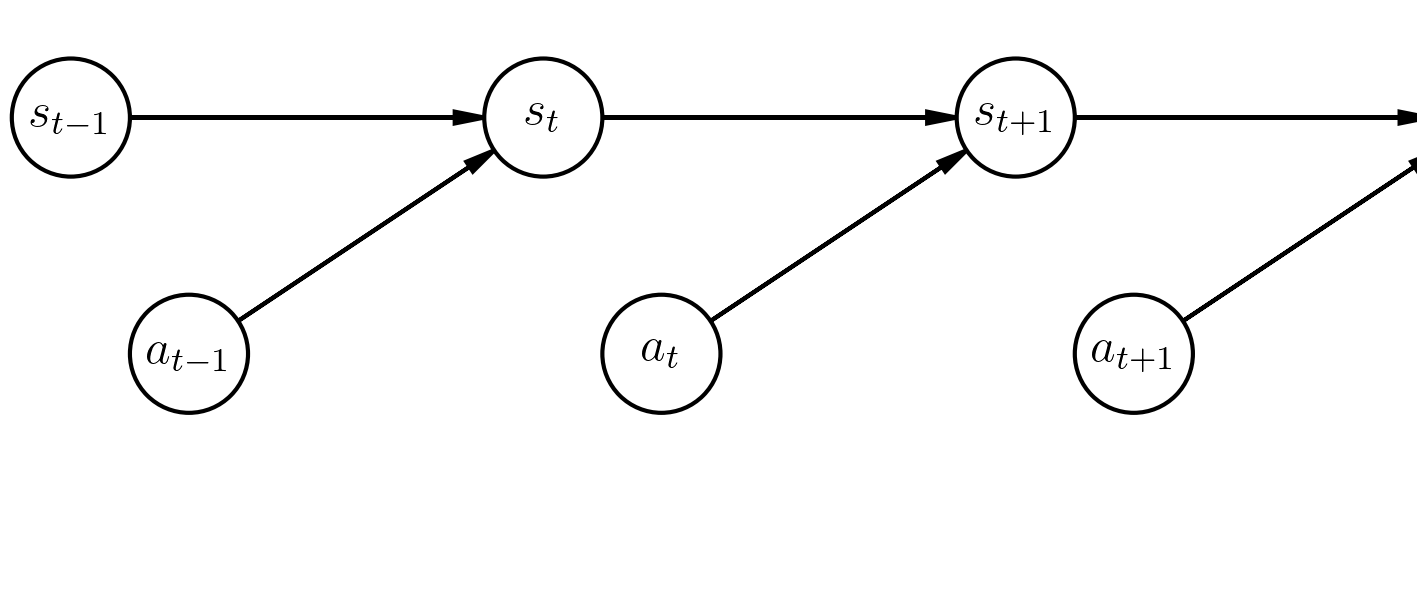
\includegraphics[scale=0.7]{pix/mdp/state_action.png}
%\caption{Lagrange乘数法}
%\label{fig:label}
\end{figure}

The graphical model has a state variable $S_t$, an action variable $A_t$ for each timestep 
$t$.

We'll define the distributions of the variables in this graphical model in a way such that 
the probability of a trajectory $\tau = (s_0, a_0, s_1, a_1, \dots s_T)$ is equal to the 
probability of the trajectory under the MDP's dynamics.

We set the distribution of $S_0$ to be $\rho(s)$ (the initial state distribution of the MDP).

For subsequent $S_t$, the distribution is defined using transition probabilities of the MDP.
$$
P(S_{t+1} = s' \vert S_{t}=s, A_t = a) = T(s' \vert a,s)
$$

The distribution for the action variables $A_t$ is uniform on the action space.
$$
P(A_t = a) = C
$$

It may seem odd that the actions are sampled uniformly, but don't worry! These are only prior 
probabilities, and we'll get interesting action distributions once we start conditioning 
(Hang tight!)

The probability of a trajectory $\tau = (s_0, a_0, s_1, a_1 , \dots s_T,a_T)$ in this model 
factorizes as
\begin{align*}
P(\tau) &= P(S_0 = s_0) \prod_{t=0}^{T-1} P(A_t = a_t)P(S_{t+1} = s_{t+1} | S_t = s_t, A_t = a_t)\\ 
&= C^T \left(\rho(s_0) \prod_{t=0}^{T-1} T(s_{t+1} \vert s_t, a_t)\right)\\  
&\propto \left(\rho(s_0)\prod_{t=0}^{T-1} T(s_{t+1} | s_t,a_t)\right) 
\end{align*}

The probability of a trajectory in our graphical model is thus directly proportional to the 
probability under the system dynamics.

In the special case that dynamics are deterministic, then 
$P(\tau) \propto 1 \{\text{Feasible}\}$ 
(that is, all trajectories are equally likely).


\subsubsection{Adding Rewards}

So far, we have a general structure for describing the likelihood of trajectories in an MDP, 
but it's highly uninteresting since at the moment, all trajectories are equally likely. To 
highlight interesting trajectories, we'll introduce the concept of {\em optimality}.

We'll say that an agent is {\bf optimal} at timestep $t$ with some probability which depends 
on the current state and action : $P(\text{Optimal at } t) = f(s_t,a_t)$. We'll embed 
optimality into our graphical model with a binary random variable at every timestep $e_t$, 
where $P(e_t = 1 \vert S_t=s_t, A_t=a_t) = f(s_t,a_t)$.

While we're at it, let's define a function $r(s,a)$ to be $r(s_t,a_t) = \log f(s_t,a_t)$. 
The notation is very suggestive, and indeed we'll see very soon that this function 
$r(s,a)$ plays the role of a reward function.

The final graphical model, presented below, ends up looking much like one for a Hidden 
Markov Model.

\begin{figure}[H]
\centering
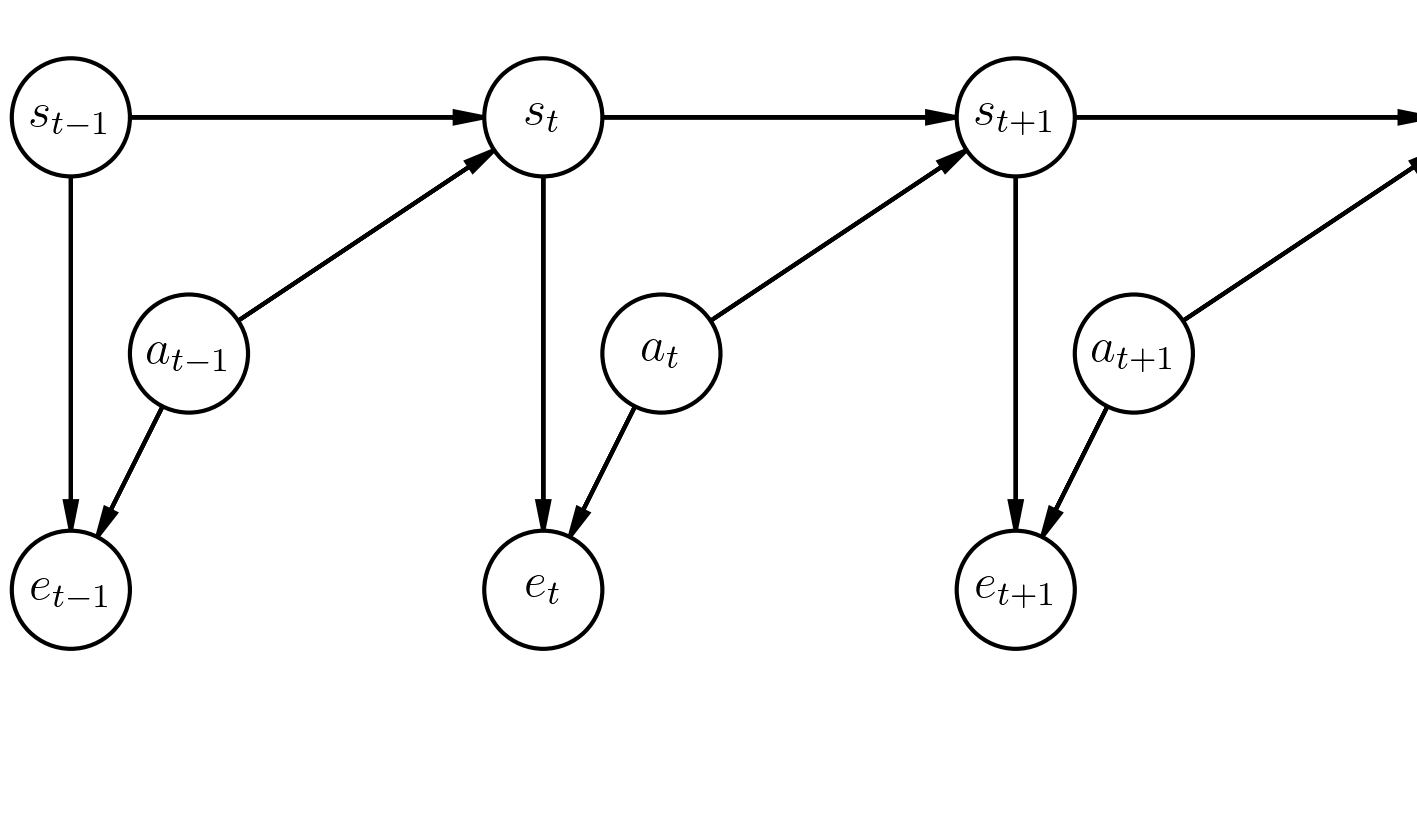
\includegraphics[scale=0.7]{pix/mdp/state_action_reward.png}
%\caption{Lagrange乘数法}
%\label{fig:label}
\end{figure}

For a trajectory $\tau$, the probability that it is optimal at all timesteps is proportional 
(exponentially) to the total reward received in the trajectory.
$$
P(\text{All } e_t=1 | \tau)  =\exp \left(\sum_{t=0}^T r(s_t,a_t)\right)
$$
{\bf PROOF}
\begin{align*}
P(\text{All } e_t=1 | \tau) 
&= \prod_{t=0}^T P(e_t = 1 \vert S_t=s_t, A_t=a_t) \\ 
&= \prod_{t=0}^T f(s_t,a_t) \\ &= \prod_{t=0}^T \exp{r(s_t,a_t)} \\ 
&=  \exp \left(\sum_{t=0}^T r(s_t,a_t)\right)
\end{align*}

We'll describe the {\bf optimal trajectory distribution} as the distribution when 
conditioned on being optimal at all time steps.
$$
\pi_{\text{optimal}}(\tau) = P(\tau \vert \text{All } e_t =1) = P(\tau~\vert~e_{1:T} = 1)
$$
Explicitly writing out this distribution, we have that
$$
P(\tau ~\vert ~e_{1:T} = 1) \propto \exp\left(\sum_{t=0}^T r(s_t,a_t)\right)P(\tau)
$$
{\bf PROOF}
\begin{align*}
P(\tau ~\vert~ e_{1:T} =1) 
&= \frac{P(e_{1:T} =1 \vert \tau)P(\tau)}{P(e_{1:T} =1)} \\ 
&\propto P(e_{1:T} =1 \vert \tau)P(\tau) \\ 
&\propto \exp\left(\sum_{t=0}^T r(s_t,a_t)\right)P(\tau)
\end{align*}
Under deterministic dynamics, since $P(\tau) \propto 1\{\text{Feasible}\}$, the probability 
of any feasible trajectory is
$$
P(\tau~\vert~ e_{1:T} =1) \propto \exp\left(\sum_{t=0}^T r(s_t,a_t)\right)
$$
This can be viewed as a special form of an energy-based model, where the energy of a 
trajectory is proportional to the reward.


%+++++++++++++++++++++++++++++++++++++++++++
\subsection{Exact Inference in the Graphical Model}

We now have a model for what the optimal trajectory distribution is, so the next appropriate 
step is to look at optimal action distributions. If I am at state $s$ on timestep $t$, what 
is the "optimal" distribution of actions?

Pedantically, this corresponds to finding
$$
\pi_{t}(a \vert s) = P(A_t = a~\vert~S_t = s,e_{1:T} =1)
$$
In our graphical model, $A_t$ is independent of all events before $t$ (
$A_t \perp E_1 \dots E_{t-1})$). We can verify this mathematically, but the intuition is 
that the distribution of actions at a timestep shouldn't be impacted by what happened 
previously (the environment is Markovian). So,
$$
\pi_{t}(a \vert s) = P(A_t = a \vert S_t = s, e_{t:T} =1)
$$
Solving for these probabilities corresponds to doing exact inference in the graphical model 
above, which looks much like the forward-backward algorithm for HMMs. The procedure goes 
as follows:
\begin{itemize}
%\setlength{\itemsep}{0pt}
%\setlength{\parsep}{0pt}
\setlength{\parskip}{0pt}
\item[1.]
{\em Backward message passing}: Compute probabilities
$P(e_{t:T} = 1 ~\vert~ S_t =s)$ and $P(e_{t:T} = 1 ~\vert~ S_t =s, A_{t} = a)$

\item[2.]
{\em Forward message passing}: Compute probabilities
$P(A_t = a \vert S_t = s, e_{t:T} =1)$ using Bayes Rule and the backwards messages.

\end{itemize}


\subsubsection{Backward Messages}

We can compute these backward messages recursively, since
\begin{itemize}
%\setlength{\itemsep}{0pt}
%\setlength{\parsep}{0pt}
\setlength{\parskip}{0pt}
\item[1.]
$P(e_{t:T} = 1\vert A_t =a, S_t=s)$ can be expressed in terms of 
$P(e_{t+1:T} = 1 \vert S_{t+1} = s')$

\item[2.]
$P(e_{t:T} = 1\vert S_t=s)$ can be expressed in terms of 
$P(e_{t:T} = 1\vert S_t=s, A_t =a)$

\end{itemize}
Working through the math (see the proof for more details)
$$
P(e_{t:T} = 1 = e^{r(s,a)} \mathbb{E}_{s' \sim T(\cdot \vert s,a)}[P(e_{t+1:T}=1 \vert S_{t+1}=s')]
$$
$$
P(e_{t:T} = 1\vert S_t=s) = \mathbb{E}_{a}[P(e_{t:T} = 1 \vert A_t=a, S_t =s)]
$$
{\bf PROOF}
\begin{align*} 
P(e_{t:T} = 1&\vert A_t =a, S_t=s)\\ &= \int_{\mathcal{S}} P(e_{t:T}=1, S_{t+1}=s' \vert S_t=s, A_t=a) ds'\\
&= \int_{\mathcal{S}} P(e_t = 1 | S_t=s, A_t=a)P(e_{t+1:T}=1, S_{t+1}=s' \vert S_t=s, A_t=a) ds'\\
&= P(e_t = 1 | S_t=s, A_t=a) \int_{\mathcal{S}} P(e_{t+1:T}=1 \vert S_{t+1}=s') P(S_{t+1} = s' \vert S_t=s, A_t=a) ds'\\
&= e^{r(s,a)} \mathbb{E}_{s' \sim T(\cdot \vert s,a)}[P(e_{t+1:T}=1 \vert S_{t+1}=s')]\\
P(e_{t:T} = 1&\vert S_t=s)\\ &= \int_{\mathcal{A}} P(e_{t:T} = 1, A_t=a \vert S_t=s) da\\
&= \int_{\mathcal{A}} P(e_{t:T} = 1 \vert A_t=a , S_t=s) P(A_t=a) da \\ 
&= \mathbb{E}_{a}[P(e_{t:T} = 1 \vert A_t=a, S_t =s)]\\
\end{align*}

That looks pretty ugly and uninterpretable, but if we view the expressions in 
log-probability space, there's rich meaning.

Let's define
$$
Q_t(s,a) = \log P(e_{t:T} = 1\vert A_t =a, S_t=s)
$$
$$
V_t(s) = \log P(e_{t:T} = 1 \vert S_t=s)
$$
$Q$  and $V$ are very suggestively named for a good reason: we'll discover that they are 
the analogue of the $Q$ and $V$ functions in standard RL. Rewriting the above expressions 
with $Q_t(\dot, \dot)$ and $V_t(\dot)$:
$$
Q_t(s,a)  = r(s,a) + \log  \mathbb{E}_{s' \sim T(\cdot \vert s,a)}[e^{V_{t+1}(s')}]
$$
$$
V_t(s) = \log \mathbb{E}_a [e^{Q_t(s,a)}]
$$
Remember that the function $\log \mathbb{E}[\exp(f(X))]$ acts as a "soft" maximum 
operation: that is
$$
\log \mathbb{E}[\exp(f(X))] = \text{soft} \max_X f(X) \approx \max_{X} f(X)
$$
We'll denote it as soft $\max$ from now on - but don't get it confused with the actual 
softmax operator. With this notation:
$$
Q_t(s,a) = r(s,a) + \text{soft} \max_{s'} V_{t+1}(s')
$$
$$
V_t(s) = \text{soft} \max_{a} Q_{t}(s,a)
$$
These recursive equations look very much like the Bellman backup equations!

These are the {\bf soft Bellman backup equations}. They differ from the traditional 
Bellman backup in two ways:
\begin{itemize}
%\setlength{\itemsep}{0pt}
%\setlength{\parsep}{0pt}
\setlength{\parskip}{0pt}
\item[1.]
The value function is a "soft" maximum over actions, not a hard maximum.

\item[2.]
The $q$-value function is a "soft" maximum over next states, not an expectation: this 
makes the $Q$-value "optimistic wrt the system dynamics" or "risk-seeking". It'll favor 
actions which have a low probability of going to a really good state over actions which 
have high probability of going to a somewhat good state. When dynamics are deterministic, 
then the $Q$-update is equivalent to the normal backup:
$Q_t(s,a) = r(s,a) + V_{t+1}(s')$

\end{itemize}
{\bf Passing backwards messages corresponds to performing Bellman updates in an MDP}, 
albeit with slightly different backup operations


\subsubsection{Forward Messages}

Now that we know that the $Q$ and $V$ functions correspond to backward messages, let's 
now compute the optimal action distribution.
\begin{align*}
P(A_t =a \vert S_t=s, e_{t:T}=1) &= \frac{P(e_{t:T}=1 \vert A_t =a,  S_t=s)P(A_t = a \vert S_t =s)}{P(e_{t:T}=1\vert S_t=s)}\\
&= \frac{e^{Q_t(s,a)}C}{e^{V_t(s)}}\\
&\propto \exp(Q_t(s,a) - V_t(s))\\
&\propto \exp(A_t(s,a))
\end{align*}
If we define the {\rm advantage} $A_t(s,a) = Q_t(s,a) - V_t(s)$, then we find that the 
optimal probability of picking an action is simply proportional to the exponentiated 
advantage!

Haarnoja et al perform a derivation similar to this to find an algorithm called Soft 
$Q$-Learning. In their paper, they show that the soft bellman backup update is a 
contraction, and so $Q$-learning with the soft backup equations have the same convergence 
guarantees that $Q$-learning has in the discrete case. Empirically, they show that this 
algorithm can learn complicated continuous control tasks with high sample efficiency. 
In follow-up works, they deploy the algorithms on robots and also present actor-critic 
methods in this framework.


%+++++++++++++++++++++++++++++++++++++++++++
\subsection{Approximate Inference with variational methods}

Let's try to look at inference in this graphical model in a different way. Instead of 
doing exact inference in the original model to get a policy distribution, we can attempt 
to learn a variational approximation to our intended distribution
$q_{\theta}(\tau) \approx P(\tau \vert e_{1:T}=1)$.

The motivation is the following: we want to learn a policy $\pi(a|s)$ such that sampling 
actions from $\pi$ causes the trajectory distribution to look as close to 
$P(\tau \vert e_{1:T} = 1)$ as possible. We'll define a variational distribution 
$q_\theta(\tau)$ as follows:
\begin{align*}
q_\theta(\tau) &= P(S_0 = s_0) \prod_{t=0}^T q_{\theta}(a_t \vert s_t) P(S_{t+1} \\
&= s_{t+1} \vert S_{t} = s_t, A_t = a_t) \\
&= \left(\prod_{t=0}^T q(a_t | s_t)\right) P(\tau)
\end{align}
This variational distribution can change the distribution of actions, but fixes the 
system dynamics in place. This is a form of structured variational inference, and we 
attempt to find the function $q_{\theta}(a \vert s)$ which minimizes the KL divergence 
with our target distribution.
$$
\min_{\theta} D_{KL}(q_{\theta}(\tau) \| P(\tau \vert e_{1:T} = 1))
$$
If we simplify the expressions, it turns out that
$$
\arg\min_{\theta} D_{KL}(q_{\theta}(\tau) \| P(\tau \vert e_{1:T} = 1)) 
= \arg \max_{\theta} \mathbb{E}_{\tau \sim q}[ \sum_{t=0}^T  r(s_t,a_t) 
+ \mathcal{H}(q_{\theta}(\cdot \vert s_t)]
$$
{\bf PROOF}
Remember from the first section that
$$
P(\tau \vert \text{All } e_t=1) = P(\tau) \exp(\sum_{t=0}^T r(s_t,a_t))
$$
\begin{align*}
D_{KL}(q_{\theta}(\tau) \| P(\tau \vert \text{All } e_t = 1)) &= -\mathbb{E}_{\tau \sim q}[\log \frac{P(\tau \vert \text{All } e_t = 1)}{q_{\theta}(\tau)}]\\
 &= -\mathbb{E}_{\tau \sim q}[\log \frac{P(\tau) \exp(\sum_{t=0}^T r(s_t,a_t))}{ P(\tau)\left(\prod_{t=0}^T q_{\theta}(a_t | s_t)\right)}]\\
 &= -\mathbb{E}_{\tau \sim q}[\log \frac{\exp(\sum_{t=0}^T r(s_t,a_t))}{\prod_{t=0}^T q_{\theta}(a_t | s_t)}]\\
&= -\mathbb{E}_{\tau \sim q}[\log \frac{\exp(\sum_{t=0}^T r(s_t,a_t))}{\exp (\sum_{t=0}^T \log q_{\theta}(a_t | s_t)}]\\
 &=  -\mathbb{E}_{\tau \sim q}[ \sum_{t=0}^T  r(s_t,a_t) - \log q_{\theta}(a_t | s_t))]\\
\end{align*}
Recalling that $-\log q(a_t | s_t)$ is a point estimate of the entropy of 
$\mathcal{H}(q(\cdot \vert s))$, we get our result.
$$
D_{KL}(q_{\theta}(\tau) \| P(\tau \vert e_{1:T} = 1)) = -\mathbb{E}_{\tau \sim q}[ \sum_{t=0}^T  r(s_t,a_t) + \mathcal{H}(q_{\theta}(\cdot \vert s_t)]
$$

The best policy $q_\theta(a|s)$ is thus the one that maximizes expected reward with 
an entropy bonus. This is the the objective for {\bf maximum entropy reinforcement 
learning}. Performing structured variational inference with this particular family 
of distributions to minimize the KL divergence with the optimal trajectory distribution 
is equivalent to doing reinforcement learning in the max-ent setting!

A cross check out can be found in \nameref{Reinforcement-Learning-eq-Reverse-KL}.
